\documentclass{article}

\usepackage[final]{nips}

\usepackage[utf8]{inputenc} % allow utf-8 input
\usepackage[T1]{fontenc}    % use 8-bit T1 fonts
\usepackage{hyperref}       % hyperlinks
\usepackage{url}            % simple URL typesetting
\usepackage{booktabs}       % professional-quality tables
\usepackage{amsfonts}       % blackboard math symbols
\usepackage{nicefrac}       % compact symbols for 1/2, etc.
%\usepackage{microtype}      % microtypography
\usepackage{amsmath}
\usepackage{bm}
\usepackage{tikz}
\usetikzlibrary{bayesnet}

\newcounter{question}
\newcommand{\question}{\stepcounter{question}\paragraph{Question \thequestion}}
\newcommand{\mat}[1]{\textbf{\textit{#1}}}

\title{Coursework 1 - Modelling}

\author{
  Jonas Osborn \\
  \texttt{jo14944} \\
  \And
  Tristan Saunders \\
  \texttt{ts16802} \\
  \And
  Corin Varney \\
  \texttt{cv14985} \\
}

\begin{document}

\maketitle

\section{The prior}
\subsection{Theory}
\question \emph{1.} As the instances of $y$ are noisy observations of the underlying process and we do not know anything about this uncertainty we can assume it is the sum of independent and identically distributed errors. The Central Limit Theorem states the distribution of the sum of a large enough number of independent, identically distributed variables will be approximately normally distributed. From this we can say that our model of $y$ has the following form:
\begin{align*}
	y & = f(x) + \epsilon \\
	\text{where:~}
	\epsilon & \sim \mathcal{N}(0, \mat{I})
\end{align*}
And so from this we have the likelihood of each $y_i$ as a Gaussian distribution with mean $f(x_i)$.\\

\emph{2.} Choosing a spherical covariance matrix for the likelihood means that we are assuming the different dimensions of $y_i$ to be independent and identically distributed. As they are independent they do not covary with each other and so the covariance matrix is diagonal. As they are identically distributed they all have the same variance. Therefore the covariance matrix is spherical.
\question
\begin{align*}
	p(\mat{Y}|f,\mat{X}) &= p(y_1,\ldots,y_{N-1},y_N|f,\mat{X}) \\
	&= p(y_N|y_{N-1},\ldots,y_1,f,\mat{X})p(y_{N-1}|y_{N-2},\ldots,y_1,f,\mat{X})\ldots p(y_1|f,\mat{X}) \\
\end{align*}
\subsubsection{Linear regression}
\question
\begin{align*}
	p(\mat{Y}|\mat{X},\mat{W}) &= \prod_{i}^Np(\mat{y}_i|\mat{x}_i,\mat{W}) \\
	&= \prod_{i}^N\mathcal{N}(\mat{W}\mat{x}_i,\sigma^2\mat{I}) \\
	&= \mathcal{N}(\mat{W}\mat{X},\sigma^2\mat{I})
\end{align*}
\question A conjugate prior is one that is conjugate to the posterior, meaning they are in the same family of distributions. A conjugate prior is useful as it gives a closed-form solution for the posterior. If we didn't choose a conjugate prior then numerical integration may be necessary to calculate the posterior which may mean the solution is potentially intractable. The conjugate prior for a Gaussian posterior is a Gaussian.
\question Just as encoding the prefrence in a $L_2$ norm is equivalent to having a Gaussian prior, encoding the preference using a $L_1$ norm is equivalent to having a Laplace prior. This is because the Laplace distribution estimates median rather than the mean estimated by the Guassian and median minimises the $L_1$ norm and mean the $L_2$

The shape of the laplace distribution's probability density function, with it's higher peak around zero compared to the probability density function of a Gaussian means that more co-efficients are likely to be equal to zero and this leads to a sparser model than those produced by a Gaussian prior.
\question
\begin{align*}
	p(\mat{W}|\mat{X},\mat{Y}) &= \frac{1}{Z}p(\mat{Y}|\mat{X},\mat{W})p(\mat{W}) \\
	&= \frac{1}{Z}\mathcal{N}(\mat{W}\mat{X},\sigma^2\mat{I})\mathcal{N}(\mat{W}_0,\tau^2\mat{I})
\end{align*}
$\frac{1}{Z}$ is the normalising constant to ensure that the posterior is a probability density function by making the area under the graph equal to $1$ this constant is called the evidence. We will ignore it for now.

By the probability density function of the multivariate normal distribution, we have:
\begin{align*}
	p(\mat{W}|\mat{X},\mat{Y}) \propto\ &\frac{1}{\sqrt{(2\pi)^N\sigma^2}}\exp\bigg(-\frac{1}{2\sigma^2}(\mat{Y}-\mat{X}\mat{W})^T(\mat{Y}-\mat{X}\mat{W})\bigg) \\
	&\cdot \frac{1}{\sqrt{(2\pi)^N\tau^2}}\exp\bigg(-\frac{1}{2\tau^2}(\mat{W}-\mat{W}_0)^T(\mat{W}-\mat{W}_0)\bigg) \\
	\propto\ &\exp\bigg(-\frac{1}{2\sigma^2}(\mat{Y}-\mat{X}\mat{W})^T(\mat{Y}-\mat{X}\mat{W})-\frac{1}{2\tau^2}(\mat{W}-\mat{W}_0)^T(\mat{W}-\mat{W}_0)\bigg) \\
	\propto\ &\exp\bigg(-\frac{1}{2\sigma^2}(\mat{Y}^T\mat{Y}-2\mat{Y}^T\mat{X}\mat{W}+\mat{W}^T\mat{X}^T\mat{X}\mat{W}) \\
	&\hspace{2.5em}-\frac{1}{2\tau^2}(\mat{W}_0^T\mat{W}_0-2\mat{W}^T\mat{W}_0+\mat{W}^T\mat{W})\bigg)
% 	&\hspace{4em}-\frac{1}{2\tau^2}(\mat{W}^T\mat{W}-2\mat{W}^T\mat{W}_0+\mat{W}_0^T\mat{W}_0)\Big) \\
% 	& \text{[TODO][UNSURE]}
\end{align*}
\begin{align*}
	p(\mat{W}|\mat{X},\mat{Y}) \propto \exp\bigg(&-\frac{1}{2\sigma^2}\mat{W}^T\mat{X}^T\mat{X}\mat{W}-\frac{1}{2\tau^2}\mat{W}^T\mat{W}	&&\mbox{quadratic term}\\
	&+\frac{1}{\sigma^2}\mat{W}^T\mat{X}^T\mat{Y}+\frac{1}{\tau^2}\mat{W}^T\mat{W}_0							&&\mbox{mixed term}\\
	&-\frac{1}{2\sigma^2}\mat{Y}^T\mat{Y}-\frac{1}{2\tau^2}\mat{W}_0^T\mat{W}_0\bigg)							&&\mbox{constant term}\\
\end{align*}
\begin{align*}
	p(\mat{W}|\mat{X},\mat{Y}) \propto \exp\bigg(&-\frac{1}{2}\mat{W}^T\Big(\frac{1}{\sigma^2}\mat{X}^T\mat{Y}+\frac{1}{\tau^2}\mat{I}\Big)\mat{W}	&&\mbox{quadratic term}\\
	&+\mat{W}^T\Big(\frac{1}{\sigma^2}\mat{X}^T\mat{Y}+\frac{1}{\tau^2}\mat{W}_0\Big)								&&\mbox{mixed term}\\
	&-\frac{1}{2\sigma^2}\mat{Y}^T\mat{Y}-\frac{1}{2\tau^2}\mat{W}_0^T\mat{W}_0\Big)								&&\mbox{constant term}\\
\end{align*}
\subsubsection{Non-parametric regression}
\question Parametric models assume that the distribution the data comes from is based on a finite, fixed set of parameters and models future predictions based off these parameters, they capture everything there is to know about the data. Non-parametric models do not make such assumptions about the model structure and instead infer structure from the data, they have parameters but these are not fixed in advance and there can be an infinite set of parameters.

Non-parametric models are more flexible and can represent a wider variety of data and will represent the data better if the assumptions made in the parametric model are incorrect but are less precise and accurate than parametric methods if the right assumptions are made.

Parametric models are often easier interpreted as they are simpler to transcribe and are also often faster to compute due to lacking the complexity and flexibility of the non-parametric models.
\question As we use a Gaussian process we define this prior over functions and want our prior to put some constraints on the space of functions. The fact that its a Gaussian process means that for an arbitary set of points $x_i, \ldots, x_j$ we assume that $p(f_i), \ldots,f(x_j))$ is jointly Gaussian with mean $0$ and covariance function $k$, from this we have the equation for our prior:
$$
	p(f|\mat{X},\bm{\theta}) = \mathcal{N}(0, k(\mat{X},\mat{X}))
$$
The covariance function $k$ allows us to set constraints from our assumptions about the mapping $f$. For example our assumption about the functions smoothness that if $x_i$ and $x_j$ are similar then we expect $f_i$ and $f_j$ to be similar too, with certain kernel functions for $f$ we can only sample functions that have sufficient smoothness by ensuring that constraint.
\question [TODO]
\question
\begin{align*}
	p(\mat{Y},\mat{X},f,\bm{\theta}) = p(\mat{Y}|f)p(f|\mat{X},\bm{\theta})p(\mat{X})p(\bm{\theta})
\end{align*}
\begin{center}
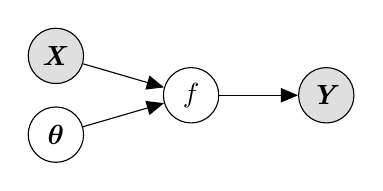
\begin{tikzpicture}
	\node[obs] (Y) {$\mat{Y}$}; %
	\node[latent, left=of Y] (f) {$f$} ; %
	\node[obs, left=of f, yshift=0.5cm] (X) {$\mat{X}$} ; %
	\node[latent, left=of f, yshift=-0.5cm] (theta) {$\bm{\theta}$} ; %
	\edge {X,theta} {f}; %
	\edge {f} {Y}; %
\end{tikzpicture}
\end{center}
[UNSURE]
\begin{itemize}
	\item $\mat{X}$ and $\bm{\theta}$ are independent
	\item $f$ is conditionally dependent on both $\mat{X}$ and $\bm{\theta}$
	\item $\mat{Y}$ is conditionally dependent on $f$ and conditionally independent of $\mat{X}$ and $\bm{\theta}$
\end{itemize}
\question This marginalization shows the likelihood of the data we have observed over all the functions constrained by the prior. [UNSURE]

There are two sources of uncertainty here, that associated with $f$ in the prior and that associated with $\epsilon$ in the likelihood, these are independent and as such are merged by simply adding to form the covariance of the marginal likelihood Gaussian.

Leaving the $\theta$ on the left-hand side of the expression implies that it has remained throughout this integral and thus the result is a function of $\theta$.
\subsection{Practical}
\subsubsection{Linear regression}
\question [TODO]
\subsubsection{Non-parametric regression}
\question [TODO]
\question [TODO]
\section{The posterior}
\subsection{Theory}
\question We make assumptions about the nature of the variables in $\mat{X}$ and encode this in ou [TODO]
\question We have encoded the assumption that all the dimensions in each variabl of $\mat{X}$ are independent as we have used a spherical Gaussian.
\question [TODO]
\subsubsection{Learning}
\question [TODO]
\subsubsection{Practical optimisation}
\question [TODO]
\subsubsection{Non-parametric}
\question [TODO]
\subsection{Practical}
\subsubsection{Linear representation learning}
\question [TODO]
\end{document}
